\documentclass[12pt,english]{article}
\usepackage{geometry}
\usepackage{float}
\usepackage{caption}
\geometry{verbose,tmargin=3cm,bmargin=3cm,lmargin=3cm,rmargin=3cm}
\usepackage{amsmath}
\usepackage{amssymb}
\usepackage{amsthm}
\usepackage{adjustbox}
\usepackage{hyperref}
\usepackage{graphicx}
\usepackage{setspace}
\usepackage{changepage}
\onehalfspacing
\usepackage{babel}
\newcommand{\expec}{\ensuremath{\mathbb E}}
\begin{document}
\begin{center}
{\Large{}Section 3: Marginal product of capital} \\
{\large{}de Mel et al (2008), de Mel et al (2009), Fafchamps et al (2013), Mckenzie (2016)}
\par\end{center}{\Large \par}

\begin{center}
EEP 152
\par\end{center}

\begin{center}
September 14, 2016
\par\end{center}

\begin{itemize}
	\setlength\itemsep{-0.5em}
	\item RCT (15 min)
	\item MPK and discussion (20 min)
	\item Mckenzie (2016) and discussion (15 min)
\end{itemize}
Copies of public versions of the four papers are available on the section Github at \href{github.com/johnloeser/eep152}{github.com/johnloeser/eep152} in the ``section3'' folder. If you missed the first two sections, it would be useful to briefly go through the section syllabus, also available on the section Github.

\section{Randomized controlled trials (RCTs)}

Let's start where we left off in class -- we're interested in estimating the marginal product of capital (MPK). Recall that the MPK is the number of \$ firm income would increase by (per unit of time) if we increased the firm's capital stock by \$1.\footnote{It's worth noting briefly that income is a flow variable, while capital is a stock variable.}

We could try a number of ways to estimate this. First, imagine using the cross-section of firms. We could look at all the firms in the US in 2016, and calculate the relationship between income and capital. If all firms had the same production function, this would work!

\begin{center}
	\begin{adjustbox}{
			max width=0.65\textwidth,
		}
		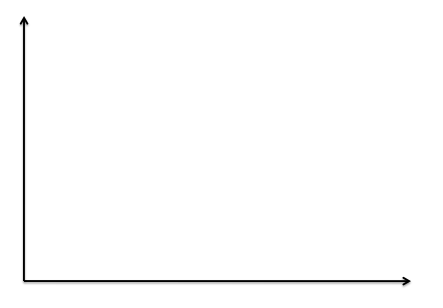
\includegraphics{axes.png}
	\end{adjustbox}
\end{center}

Unfortunately, the production function likely varies across firms for a large number of reasons. For example, some firms might be more productive than others. If this is the case, we might estimate something very different from MPK.

\begin{center}
	\begin{adjustbox}{
			max width=0.65\textwidth,
		}
		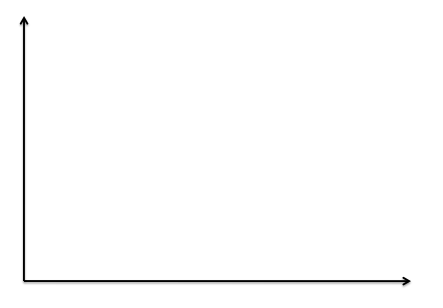
\includegraphics{axes.png}
	\end{adjustbox}
\end{center}

Second, we could look within firm over time. We could look at firms levels of income and capital in 2015 and 2016, and see how much firm income increases by when capital increases. This also seems like it would work!

\begin{center}
	\begin{adjustbox}{
			max width=0.65\textwidth,
		}
		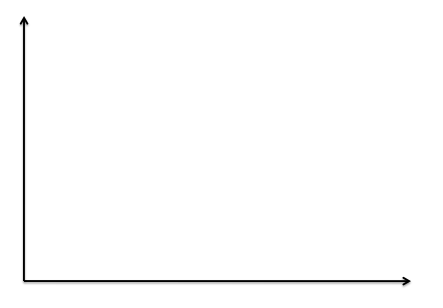
\includegraphics{axes.png}
	\end{adjustbox}
\end{center}

However, the problem is that firms that experience large increases in capital are likely very different from firms that do not. For example, those might likely be the exact firms that increased a productivity increase!

\begin{figure}[H]
	\begin{minipage}{.5\textwidth}
		\centering
		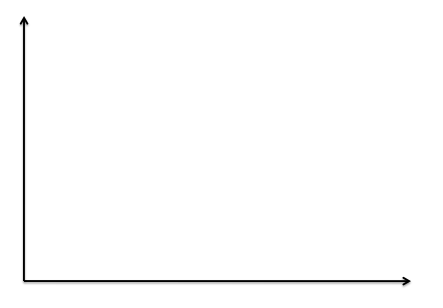
\includegraphics[width = \textwidth]{axes.png}
	\end{minipage}
	\begin{minipage}{.5\textwidth}
		\centering
		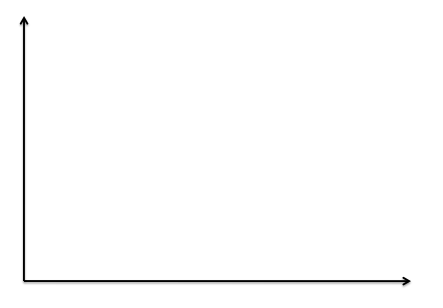
\includegraphics[width = \textwidth]{axes.png}
	\end{minipage}
\end{figure}

A third thing we could try is to look for a plausibly random source of variation in the amount of capital firms have. Even better, we could randomly assign increases in capital to some firms, and compare the increases in income those firms experience to the firms which did not receive increases in capital.

\begin{figure}[H]
	\begin{minipage}{.5\textwidth}
		\centering
		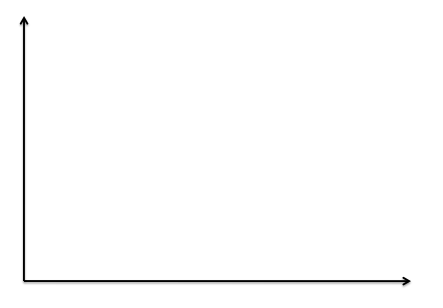
\includegraphics[width = \textwidth]{axes.png}
	\end{minipage}
	\begin{minipage}{.5\textwidth}
		\centering
		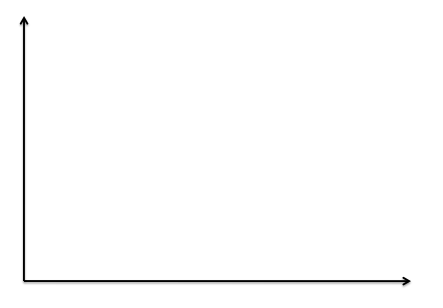
\includegraphics[width = \textwidth]{axes.png}
	\end{minipage}
\end{figure}

This will in fact allow us to estimate MPK. However, the central question is the same as the question we asked with Schofield (2014) and Schilbach (2015) last section -- what can we learn from this?

\section{Marginal product of capital (MPK)}

The first three papers listed above -- ``Returns to capital in microenterprises: Evidence from a field experiment'' (de Mel et al (2008)), ``Are women more credit constrained? Experimental evidence on gender and microenterprise returns'' (de Mel et al (2009)), and ``Microenterprise growth and the flypaper effect: Evidence from a randomized experiment in Ghana'' (Fafchamps et al (2013)) -- use RCTs to estimate the MPK in Ghana and Sri Lanka. In particular, they focus on extremely small firms (mean monthly profits are about \$120 in Ghana and \$50 in Sri Lanka) with no employees.

This is an interesting population of firms (generally called ``microenterprises'') because they likely do not have access to formal credit. This may create a poverty trap -- if these firms had formal credit, they could borrow, invest and grow, but they can't get access to formal credit until they're sufficiently large.

\begin{center}
	\begin{adjustbox}{
			max width=0.65\textwidth,
		}
		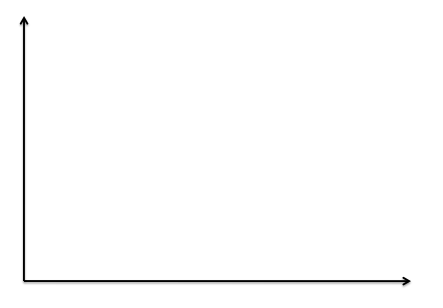
\includegraphics{axes.png}
	\end{adjustbox}
\end{center}

To test this, firms are randomly given grants, in-kind transfers of capital, or nothing, and profits are measured before and after randomization. MPK is calculated by diving the increase in income in the treatment groups (those receiving grants or in-kind transfers) relative to the control groups (those receiving nothing) by the increase in capital in the treatment groups relative to the control groups.

$$ \text{MPK} = \frac{(\pi_{T1} - \pi_{T0}) - (\pi_{C1} - \pi_{C0})}{(K_{T1} - K_{T0}) - (K_{C1} - K_{C0})} $$

A few key facts are documented:
\begin{enumerate}
	\item Estimated MPK is high - roughly 6\%/month in Sri Lanka and 15\% in Ghana
	\begin{enumerate}
		\item It is hard to explain this without some sort of constraint -- otherwise, if you could spend \$1 on capital today and increase your profit over the next year by \$0.72/\$1.80, you probably would
	\end{enumerate}
	\item Profits of female headed microenterprises do not respond to cash grants, but appear to respond to in-kind grants
	\begin{enumerate}
		\item In Ghana, this is mostly driven by female headed microenterprises with low initial profits, for which the cash grants appear to be diverted to household expenditures
		\item In Sri Lanka, women receiving large cash grants appear to respond in ways to protect the expenditures from being captured by the household (spending on inventory instead of capital)
	\end{enumerate}
	\item In Sri Lanka, negative spillovers are documented -- the increases in firm profits appear to be cancelled out by a decrease in profits of other local firms (although spread out across multiple firms)
\end{enumerate}

Taken together, how do we want to interpret these results? We've mentioned in class some of the contraints that microenterprises likely face. We can see that some of these constraints are likely important, since absent constraints these firms should grow. Why don't they? It's useful to recall the story of the \textit{dosa} cookers in India from ``Economic lives of the poor''. Does this help explain poverty gaps or make them more mysterious? Can there be poverty traps at the societal level but not individual level, or at the individual level but not societal level?

\section{McKenzie (2016)}

If small grants allow us to estimate the MPK, this tells us about the slope of the production function for those firms, but not as much about the shape.\footnote{Although, using a model and some reasoning, we can try to infer about the shape.}

\begin{center}
	\begin{adjustbox}{
			max width=0.65\textwidth,
		}
		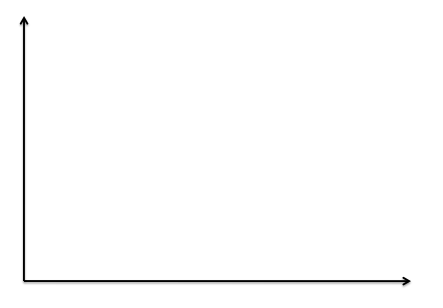
\includegraphics{axes.png}
	\end{adjustbox}
\end{center}

What if we want to know more about the production function for high levels of capital? If we're interested in societal increases in income, microenterprises might not be the right set of firms to focus on, since these firms are much less characteristic of employment in rich countries (and as countries become richer, microenterprises tend to become less relevant). Where do these medium and large firms come from? Do they drive economic growth, or does economic growth drive the emergence of medium and large firms?

``Identifying and spurring high-growth entrepreneurship: Experimental evidence from a business plan competition'' (McKenzie (2016)) used a business plan competition to study the emergence of medium sized firms. If you're interested in this paper, David McKenzie is presenting it in the Development Seminar (Evans 648, Monday, September 19, 4:00pm - 5:30pm), and he'll do it better justice (and you'll get to see a bunch of grad students and professors critiquing it).

McKenzie motivates this by documenting that 0.4\% of firms in Nigeria have at least 10 employees. For contrast, 2\% of firms in the USA have at least 20 employees. Although this doesn't sound dramatic, this translates into enormous differences in the share of the population that is self-employed. There are also reasons to think this difference might have a causal effect on the poverty gap -- large firms are easier to tax, there may be increasing returns to scale, self-employment is extremely risky, \ldots Why don't more firms have at least 10 employees in Nigeria? Constraints might be a reason, but the previous papers don't allow us to test that -- a \$100 does not approach the amount of capital a microenterprise would need to grow to that size, nor do microentrepreneurs necessarily have the greatest capacity to grow a firm to scale.

Instead, McKenzie randomly distributes \$50,000 grants to semi-finalists in a business plan competition in Nigeria. Dramatically, individuals not receiving a grant have an 11\% chance of employing 10 or more workers 1.5 years after the experiment, compared to a 34\% chance in the treatment group. Once again, this is consistent with these individuals facing constraints. A similar result in the US seems less likely -- losers of one competition can often find sources of credit from another, especially given that the final survey was more than 3 years after the initial application to the competition.

How do we interpret this? This is clearly an extremely selected sample of entrepreneurs (semifinalists in a national competition in a country with almost 200 million people), but that begs the question why these entrepreneurs don't have other sources of credit. Is misallocation of resources important in explaining poverty gaps? Why would this be less of a problem in rich countries than in poor countries? Should we worry about negative spillovers in this context as we found in Sri Lanka? Why/why not? What do we learn from this paper, and what questions does it suggest?

\end{document}